\section{Method}
\label{sec:method}

    \subsection{Preliminaries}
    \label{sec:preliminaries}
    Flow matching models learn to transport samples from a simple noise distribution to the data distribution by modeling a continuous-time probability path. Our approach builds on rectified flows \citep{liu2022flow, albergo2023buildingnormalizingflowsstochastic, fmgen}, which constructs straight-line trajectories between noise and data.%, enabling efficient and stable training.

    Let $\mathbf{x}_0 \in \mathbb{R}^{N \times C}$ denote clean data represented as a sequence of $N$ tokens, each of dimension $C$. This formulation naturally accommodates diverse input modalities, including
    image patches, video frames, and audio segments. We define a probability path by linearly interpolating between a noise distribution $\mathbf{x}_1 \sim \mathcal{N}(\mathbf{0}, \mathbf{I})$ and the data
    distribution:
    \begin{equation}
    \mathbf{x}_t = (1-t)\mathbf{x}_0 + t\mathbf{x}_1, \quad t \in [0, 1],
    \end{equation}
    where $t$ parameterizes the interpolation, with $t=1$ corresponding to pure noise and $t=0$ corresponding to clean data. The velocity field along this path is given by
    $\mathbf{v}_t = \frac{d\mathbf{x}_t}{dt} = \mathbf{x}_1 - \mathbf{x}_0.$
    A neural network $f_\theta(\mathbf{x}_t, t)$ is trained to predict the velocity field by minimizing:
    \begin{equation}
    \label{eq:flowloss}
    \mathcal{L}_{\text{gen}} = \mathbb{E}_{\mathbf{x}_0, \mathbf{x}_1, t} \| f_\theta(\mathbf{x}_t, t) - (\mathbf{x}_1 - \mathbf{x}_0) \|^2,
    \end{equation}

    where $t \sim p(t)$ denotes the timestep sampling distribution (see App.~\ref{suppsubsec:aets}). At inference, generation proceeds by solving the ordinary differential equation (ODE) $\frac{d\mathbf{x}_t}{dt} =
    f_\theta(\mathbf{x}_t, t)$ from pure noise $\mathbf{x}_1 \sim \mathcal{N}(\mathbf{0}, \mathbf{I})$ backwards in time to $t=0$, yielding a sample from the learned data distribution.

    Recent works~\citep{repa,repae,sra} demonstrate that flow matching training benefits substantially from feature alignment. Given representations from a teacher
    model $r_\phi$, these methods augment training with an auxiliary objective:
      \begin{equation}
    \mathcal{L}_{\text{rep}} = -\mathbb{E}_{\mathbf{x}_0, \mathbf{x}_1,  t, t'} \; \text{sim} \left( h_\theta^{(l)}(\mathbf{x}_t, t), r_\phi^{(k)}(\mathbf{x}_{t'}, t') \right),
    \label{eq:feature_loss}
    \end{equation}
where $\text{sim}$ denotes a similarity metric, $l$, $ k$ denote layer indices of the flow model and teacher, respectively, and $h_\theta^{(l)}(\mathbf{x}_t, t) = h_{\theta} (f_\theta^{(l)}(\mathbf{x}_t, t))$ is an MLP projection head. This loss aligns the features at the $l$-th layer of the flow model $f_\theta$ with the representation features $r_\phi^{(k)}(\mathbf{x}_{t'}, t')$ from layer $k$. 
Alignment methods achieve optimal performance when aligning with an external pretrained encoder, with DINOv2-B~\citep{dinov2} being the
predominant choice~\citep{repa,repae,irepa}. However, existing evaluations focus primarily on class-conditional ImageNet generation~\citep{imagenet}, a dataset heavily
represented in DINOv2 training, potentially biasing the reported results. In this work, we demonstrate that reliance on external models leads to unexpected behavior across data distributions, model scales, and modalities.

\begin{figure}[t]
    \centering
    \begin{subfigure}[t]{0.49\linewidth}
      \centering
      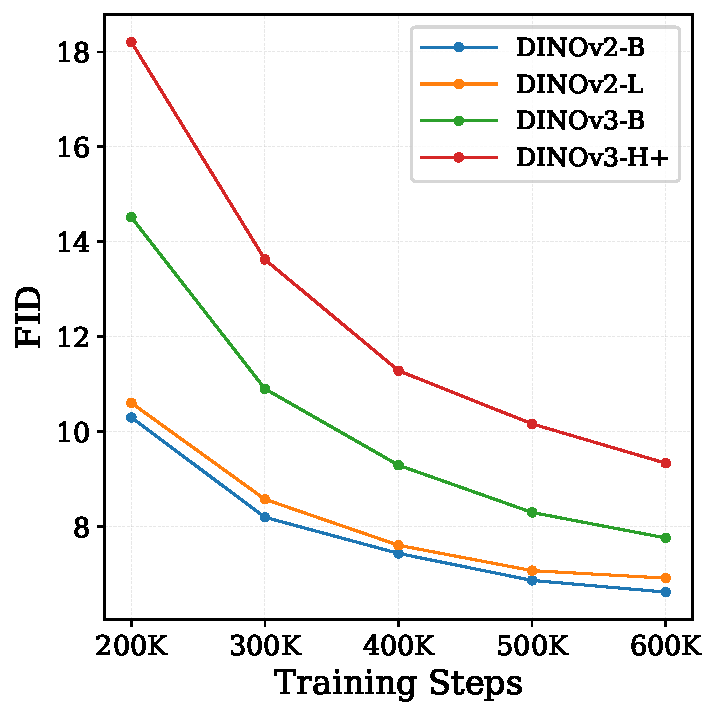
\includegraphics[width=\linewidth]{figures/repa_scaling_v2.pdf}
      \caption{REPA scaling}
      \label{fig:dino_scaling}
    \end{subfigure}
    \hfill
    \begin{subfigure}[t]{0.49\linewidth}
      \centering
      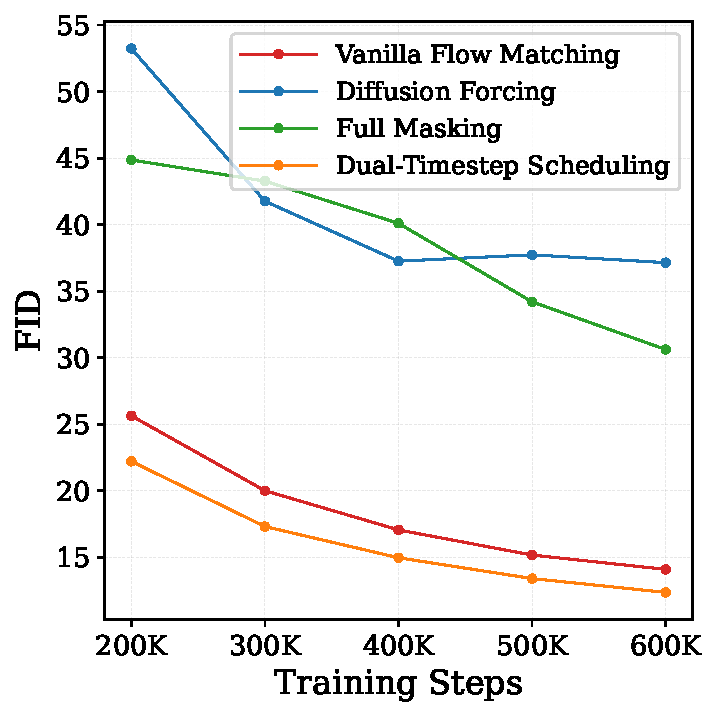
\includegraphics[width=\linewidth]{figures/noise_scheduling_v2.pdf}
      \caption{Noise scheduler comparison}
      \label{fig:dual_timestep}
    \end{subfigure}
    \caption{\textbf{Motivation.} (a) Scaling DINO (v2-B$<$ v2-L$<$ v3-H+) paradoxically degrades the generations quality using REPA. (b) Diffusion forcing and full masking create a train-inference gap which degrades generations. Our Dual-Timestep Scheduling improves generation even without a self-supervised objective.}
    \label{fig:motivation}
    \vspace{-14px}
\end{figure}

\begin{figure*}
  \centering
    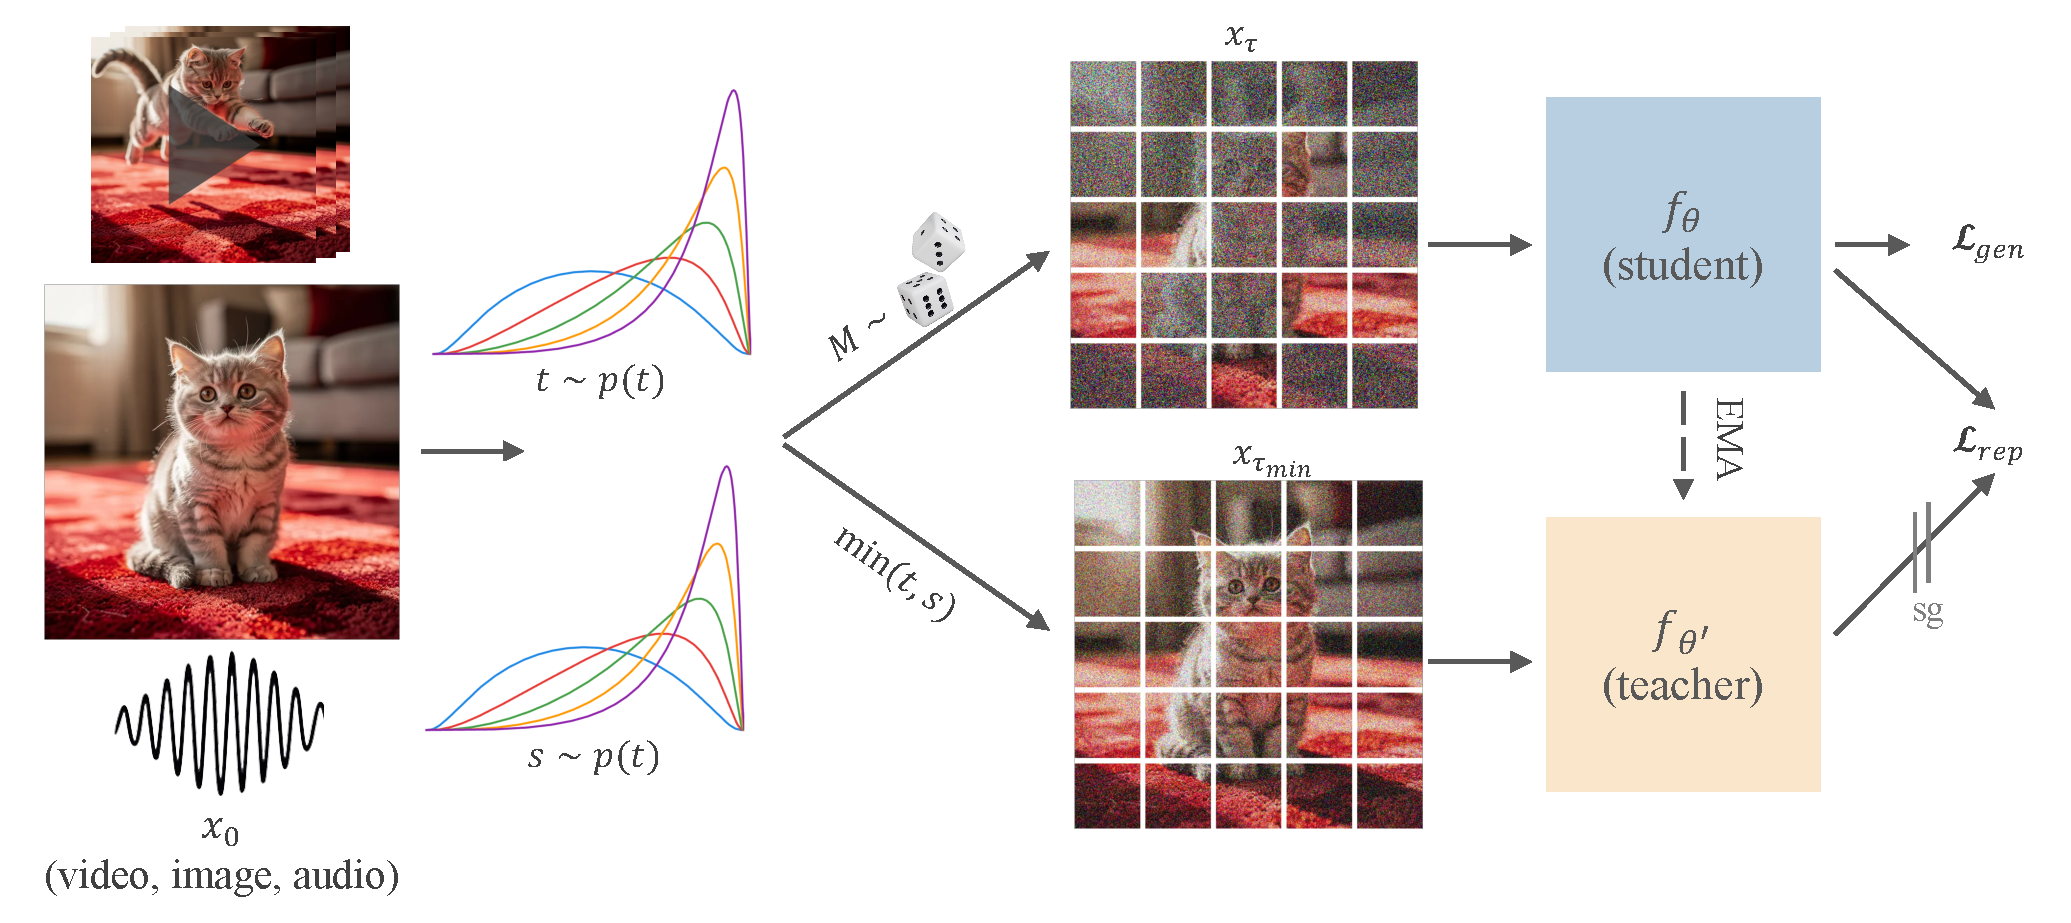
\includegraphics[width=0.90\linewidth]{figures/architecture.pdf}
    \vspace{-8px}
  \caption{\textbf{Illustration of our method.}
  Given a clean input $x_0$, we draw two timesteps $t, s$, and a random mask $M$, then noise each token according to its assigned timestep. The teacher input is noised with $\tau_{min}=\min\{t,s\}$, creating an information asymmetry compared to the student. The student is trained to simultaneously denoise the input and reconstruct the teacher's features given its mixed-noised view. 
  }
  \label{fig:method}
  \vspace{-12px}
\end{figure*}

\subsection{Motivation}
\label{sec:motivation}
We begin by presenting experiments that motivate our unified framework by testing the scaling laws of external alignment methods. Following the setup of REPA~\cite{repa} (Eq.~\ref{eq:feature_loss}), we replace the DINOv2-B backbone with increasingly stronger variants (DINOv2-L, DINOv3-B, DINOv3-H+).
Figure~\ref{fig:dino_scaling} reveals an inverse correlation: stronger representation learners consistently degrade generation quality. DINOv2-B, the smallest and weakest variant, achieves the best FID, while the most capable model, DINOv3-H+, performs the worst.
This suggests that external alignment creates a bottleneck: the generative model becomes dependent on a fixed external representation that may not align with the generative goal. Instead of relying on fixed representations, we want to strengthen them within the generative framework itself.

\subsection{Dual-Timestep Scheduling}
\label{sec:dual_timestep}

In standard flow matching, uniform noise is applied to all tokens, resulting in a denoising task that can often be solved by local correlations alone. To encourage the learning of stronger, more global representations across the model, we introduce information asymmetry: by applying different noise levels to different tokens, the model is encouraged to use cleaner tokens to infer noisy tokens. The key challenge is how to introduce such heterogeneous noise without disrupting the underlying generative dynamics.

One intuitive strategy is to randomly set $t=1$ for a subset of tokens, fully masking them. Another is to sample an independent noise level for each token, similar to diffusion forcing~\cite{chen2024diffusion}. In Fig.~\ref{fig:dual_timestep}, we compare these approaches with vanilla flow matching and our proposed scheduling method. Both naive masking and diffusion forcing substantially degrade the generation quality. We attribute this to a train--inference gap: during inference, the model must denoise uniformly noised inputs at both low and high noise levels, a regime that is rarely encountered during training.


To address this mismatch, we propose Dual-Timestep Scheduling.
The core idea is to sample \emph{two} timesteps from the noise distribution (Fig.~\ref{fig:method}). The higher of the two noises effectively corrupts information, while the cleaner one serves as context. Specifically, given an input $x_0$ we:

\begin{enumerate}
    \item Sample two timesteps: $t, s \sim p(t)$
        \item Sample a mask ${M} = \{ i \in \{1, \dots, N\} \mid u_i < \mathcal{R}_{M} \}$, with $u_i \stackrel{\text{iid}}{\sim} \mathcal{U}(0, 1)$ and a masking ratio $\mathcal{R}_{M} \leq 0.5$.
    \item 
    Construct a Dual-Timestep $\boldsymbol{\tau} \in \mathbb{R}^{N}$ to noise $\mathbf{x}_0$:
\end{enumerate}
\begin{equation}
{\tau}^i = \begin{cases}
        s & \text{if }i \in {M} \\
        t & \text{otherwise}
        \end{cases}
\end{equation}
    \begin{equation}
        \mathbf{x}_{\boldsymbol{\tau}} =  \operatorname{diag} ( \mathbf{1} - \boldsymbol{\tau}) \mathbf{x}_0 + \operatorname{diag} ( \boldsymbol{\tau} )  \mathbf{x}_1
      \end{equation}
This approach strikes a balance between vanilla homogeneous noising, which fails to encourage strong global relations, and the fully heterogeneous approach which fails to simulate inference behavior during training, while maintaining the marginal timestep distribution per token.

Interestingly, as observed in Fig.~\ref{fig:dual_timestep}, Dual-Timestep Scheduling alone, applied to the vanilla flow matching training, is able to slightly improve the generation quality even without an explicit self-supervised objective. Intuitively, this can be attributed to the presence of cleaner information in the input, which helps the model perform the denoising task, thus the model is implicitly encouraged to consider global relations, which in turn improves its generative capabilities.

\subsection{Self-Flow}
\label{ref:self_flow}
Next, we show how to leverage the information asymmetry created by Dual-Timestep Scheduling to encourage the model to learn stronger representations. 
As illustrated in Fig.~\ref{fig:method}, we maintain two models: a student network $f_\theta$ that learns from heterogeneously noised inputs $\mathbf{x}_{\boldsymbol{\tau}}$, and an EMA teacher network $f_{\theta'}$ that has the advantage of observing the cleaner $\mathbf{x}_{{\tau}_{\min}}$ which is noised by $\tau_{\min} = \min(\boldsymbol{\tau}) \in \{t, s \}$.
Based on this setup, we can now devise a feature alignment loss where the student learns to reconstruct the teacher's features from its partial, corrupt view of the input.
Formally, our representation alignment objective is given by using the teacher network $f_{\theta'}$ as the representation network and integrating the dual timestep $\boldsymbol{\tau}$ into Eq. \ref{eq:feature_loss}, using cosine similarity as the alignment metric:
\begin{equation}
\hspace{-5pt}
\mathcal{L}_{\text{rep}} = -\mathbb{E}_{\mathbf{x}_0, \mathbf{x}_1, \boldsymbol{\tau}} \cos \left(h_\theta^{(l)}(\mathbf{x}_{\boldsymbol{\tau}}, \boldsymbol{\tau}), f_{\theta'}^{(k)}(\mathbf{x}_{{\tau}_{\min}}, {\tau}_{\min}) \right) \hspace{-1pt}
\label{eq:representation_loss}
\end{equation}
Following the insights from~\citet{repa,sra} on the evolution of semantic features in diffusion models, we choose $l < k$.

To perform this task, the student is encouraged to actively leverage the cleaner tokens to infer the representations for the noisier tokens, forming global connections that transcend simple locality.
Our training objective combines generation and representation learning, parametrized by a scaling factor $\gamma$:
\begin{equation}
    \label{eq:loss}
    \mathcal{L} = \mathcal{L}_{\text{gen}} + \gamma \cdot \mathcal{L}_{\text{rep}}
\end{equation}